\documentclass[utf8]{beamer}
\usetheme{Antibes}
\usepackage[T1]{fontenc}
\usepackage{tikz}
\usepackage{caption}
\usepackage{url}
\usepackage{listings}
\usepackage{color}

\lstset{
language=C++,                % choose the language of the code
basicstyle=\footnotesize,       % the size of the fonts that are used for the code
numbers=left,                   % where to put the line-numbers
numberstyle=\footnotesize,      % the size of the fonts that are used for the line-numbers
stepnumber=1,                   % the step between two line-numbers. If it is 1 each line will be numbered
numbersep=5pt,                  % how far the line-numbers are from the code
backgroundcolor=\color{white},  % choose the background color. You must add \usepackage{color}
showspaces=false,               % show spaces adding particular underscores
showstringspaces=false,         % underline spaces within strings
showtabs=false,                 % show tabs within strings adding particular underscores
frame=single,           % adds a frame around the code
tabsize=2,          % sets default tabsize to 2 spaces
captionpos=b,           % sets the caption-position to bottom
breaklines=true,        % sets automatic line breaking
breakatwhitespace=false,    % sets if automatic breaks should only happen at whitespace
escapeinside={\%*}{*)}          % if you want to add a comment within your code
}

% Postavljanje fonta
\if@fonttimes\RequirePackage{times} \fi
\if@fontlmodern\RequirePackage{lmodern} \fi

\usecolortheme{beaver}

\newcommand{\engl}[1]{(engl.~\emph{#1})}

\title[Projekt]{Kapacitativni problem usmjeravanja vozila iz višebrojnih skladišta}
\author{Krešimir Baksa, Mihael Šafarić i Matija Šantl}

\institute{Heurističke metode optimizacije\\*Fakultet elektrotehnike i računarstva}
\date{Zagreb, siječanj 2015.}
\begin{document}

\begin{frame}
\titlepage
\end{frame}

% zadatak
\section{Projektni zadatak}
\begin{frame}
\frametitle{Definicija problema}
Kapacitativni problem usmjeravanja vozila iz višebrojnih skladišta sastoji se od odabira skladišta i pronalaska Hamiltonovih ciklusa minimalne težine u težinskom grafu, poštujući kapacitativna ograničenja ciklusa na način da su svi čvorovi posluženi. Cilj je pronaći skup skladišta koje je potrebno otvoriti i ruta koje je potrebno obići kako bi se minimizirao ukupni trošak usmjeravanja paketa do korisnika (trošak otvaranja skladišta i ruta te trošak svih odabranih ruta).
\end{frame}

\begin{frame}
\frametitle{Zadana instanca problema\footnote{crveno su označena skladišta, a plavo korisnici}}
\begin{center} 
  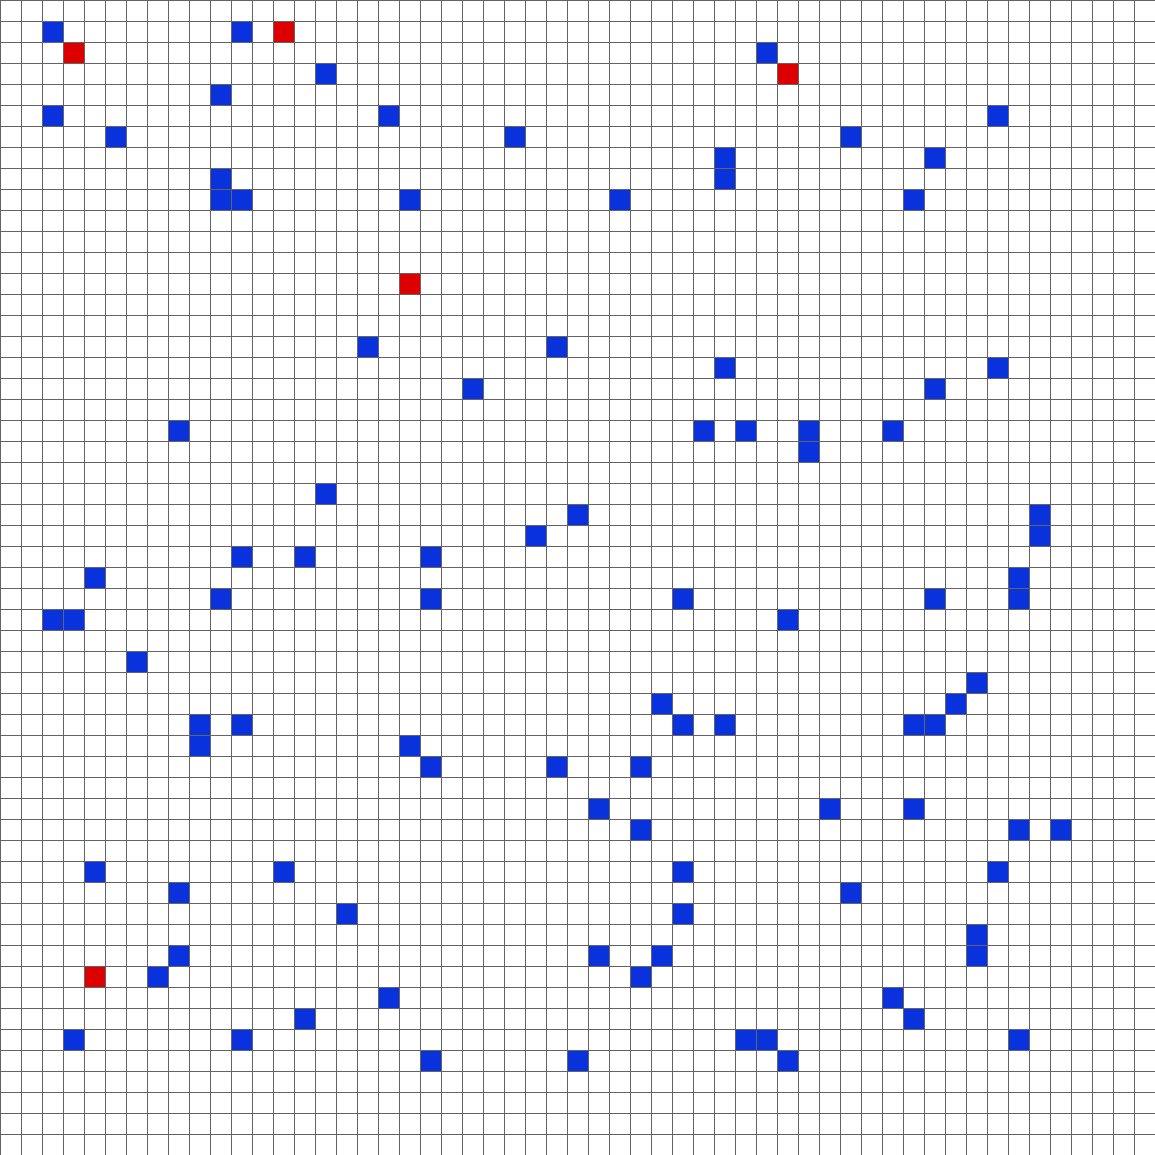
\includegraphics[height=0.8\textheight]{media/hmp-grid.png} 
\end{center} 
\end{frame}

\section{Rješenje}
\begin{frame}
\frametitle{Pristup rješavajnu}

Ovom smo problemu odlučili pristupiti na dva načina:
\vspace{5mm}
\begin{itemize}
	\item Genetskim algoritmom
	\vspace{5mm}
	\item Pohlepnim algoritmom
\end{itemize}

\end{frame}

\subsection{Genetski algoritam}
\begin{frame}
\frametitle{Jedinka}
Jedinka je predstavljena kao niz vektora, gdje vektor s indeksom \textit{i} odgovoara skladištu s indeksom \textit{i}, dok su značajke vektora \textit{i} indeksi korisnika za kojeg je to skladište zaduženo.

\vspace{5mm}

Uz niz vektora, \textit{Jedinka} također pamti svoj rezultat (\textit{fitness}) zbog njegove složenosti izračuna.

\end{frame}

\begin{frame}[fragile]{Jedinka}
\begin{lstlisting}
class Jedinka {
        private:
            std::vector<User> skladiste[NUM_WAREHOUSE];
            int fitness;

        public:
            int getFitness(void) const;
            std::vector<User> getWarehouseUsers(const int &warehouse) const;

            void setFitness(const int &_fitness);
            void setWarehouseUser(const int &warehouse, const User &user);

            void updateFitness(const std::vector<Warehouse> &w, int capacity, int cost);
};
\end{lstlisting}
\end{frame}

\begin{frame}
\frametitle{Početna populacija}

Početna populacija je pseudo-slučajna ali se pazi da bude ispravna. Prilikom slučajnog dodijeljivanja korisnika skladištu, pazi se da se ne prekorači kapacitet skladišta. Dodatno, nasumičan je odabir umanjen uvođenjem vjerojatnosti izbora skladišta koja su bliža korisniku.

\vspace{5mm}

Parametar veličine početne populacije zadaje se prilikom pokretanja programa, a podrazumijevani iznos je 100.

\end{frame}

\begin{frame}
\frametitle{Selekcija}

Korištena je troturniska selekcija s elitizmom. Sudionici troturniske selekcije se odabiru slučajno.

\vspace{5mm}

Parametar eliminacije se zadaje prilikom pokretanja programa, a podrazumijevani iznos je 25.

\end{frame}

\begin{frame}
\frametitle{Križanje}

Za jedinke $A$ i $B$, slučajno odabiremo dva indeksa $X$ i $Y$ te gradimo novu jedinku na način da od prve jedinke, $A$, uzimamo korisnike koji pripadaju skladištima iz intervala $[0, X]$ i $[Y, BROJ\_SKLADISTA]$, dok od druge jedinke, $B$, uzimamo korisnike koji pripadaju skladištima iz intervala $[X, Y]$. 

\vspace{5mm}

Ako tako nastala jedinka narušava kapacitet nekog skladišta ponavljamo postupak.

\end{frame}

\begin{frame}
\frametitle{Mutacija}

Za slučajno odabrana skladišta $X$ i $Y$, slučajnim odabirom uzmi korisnika $Z$ iz skladišta $X$ te ga probaj staviti u skladište $Y$ ako time ne narušavamo kapacitet skladišta $Y$.

\vspace{5mm}

Parametar mutacije se zadaje prilikom pokretanja programa, a podrazumijevani iznos je 25\%.

\end{frame}

\begin{frame}
\frametitle{Fitness}

Dobrotu jedinke računamo na sljedeći način:
\begin{itemize}
	\item za svako skladište, koristeći pohlepni algoritam, dodijelimo vozila za neki skup korisnika sve dok ne zadovoljimo sve korisnike (\textit{dist\_fit} funkcija)
	
	\item za svaku rutu vozila, grubom silom izračunamo najkraći Hamiltonov ciklus (\textit{bitonic\_tour\_brute}) te njegovu cijenu (\textit{bitonic\_tour\_cost} funkcija)
	
	\item tako dobivene troškove pozbrajamo i spremamo u jedinku
\end{itemize}

\end{frame}

\begin{frame}[fragile]{Fitness}
\begin{lstlisting}
int res = 0;
for (int i = 0; i < NUM_WAREHOUSE; ++i) {
  if (skladiste[i].size() > 0) {
    vector<vector<User> > tours = dist_fit(skladiste[i], capacity);
    for (int j = 0; j < (int)tours.size(); ++j) {
       vector<User> tour = bitonic_tour_brute(tours[j], w[i]);
       res += cost;
       res += bitonic_tour_cost(tour);
      }
        
      res += w[i].getCost();
    }
}
\end{lstlisting}
\end{frame}

\subsection{Pohlepni algoritam}
\begin{frame}
\frametitle{Pohlepni algoritam}

Pohlepni algoritam nakon učitavanja podataka razvrstava korisnike po skladištima na način da u trenutnom koraku minimizira trošak trenutnog korisnika do njemu najbližeg iz skladište u koje ga pokušava staviti uz dodatak troška povratka od tog korisnika do skladišta. Ako skladište u tom trenutku nema ni jednog korisnika, cijeni se dodaje trošak otvaranja skladišta.

\vspace{5mm}

To radi tako dugo dok ne razvrsta sve korisnike.

\end{frame}

\begin{frame}[fragile]{Početno rješenje}
\begin{lstlisting}
dok ima nereazvrstanih korisnika X:
  za svako skladiste Y:
    za svakog korisnika Z u skladistu Y:	
		
      cijena = udaljenost(X, Z) + udaljenost(X, Y)
			
      ako je skladiste Y prazno:
        cijena += cijena otvaranja skladista Y
		
      ako je  cijena najmanja do sad:
        W = Y
	
      stavi korisnika X u skladiste W
\end{lstlisting}
\end{frame}

\begin{frame}
\frametitle{Mutacija}

Nakon dobivanja početnog rješenja, napravi se $POPULACIJA$ broj kopija tog rješenja, te se nad svakim od njih radi mutacija koja je opisana kod genetskog algoritma.

\vspace{5mm}

Ukoliko je mutirano rješenje bolje od trenutnog, ono se zamjenjuje u populaciji.

\vspace{5mm}

Taj se postupak ponavlja $ITERACIJA$ broj puta.

\end{frame}

\begin{frame}[fragile]{Mutacija}
\begin{lstlisting}
ponovi ITERACIJA broj puta:
  za svako rjesenje R iz populacije:
    slucajno odaberi skladiste X
    slucajno odaberi skladiste Y
    slucajno odaberi korisnika A iz skladista X
		
    ako prebacivanje A iz X u Y narusava ogranicenja:
      ponovi odabir skladista i korisinka
    inace:
      prebaci korisnika A iz X u Y
      spremi izmjenjeno rjesenje
\end{lstlisting}
\end{frame}

\begin{frame}
\frametitle{Lokalna pretraga}

Nakon što smo dobili $POPULACIJA$ broj mutiranih rješenja, nad svakim od njih se pokreće postupak lokalne pretrage. 

\vspace{5mm}

Postupak lokalne pretrage, odabire par korisnika $A$ i $B$, te zamjenjuje njihova skladišta. Ako je rješenje ne narušava kapacitet ni jednog skladišta, spremamo ga u red te nastavljamo lokalnu pretragu sa sljedećim rješenjem iz reda.

\vspace{5mm}

Postupak radimo tako dugo dok ima rješenja u redu ili napravimo $limit$ broj iteracija.

\end{frame}

\begin{frame}[fragile]{Lokalna pretraga}
\begin{lstlisting}
dodaj rjesenje X u red Q

ponovi LIMIT broj puta ili dok ne konvergira:
  rjesenje R = prvo rjesenje iz reda Q
  za svaki par korisnika (A, B):
    ako zamjenom skladista korisnika A i B u R ne narusavao ogranicenja:
      R` = zamjeni skladista korisnika A i B
      
      ako je R` bolje od X:
        X = R`
      
      ako je trenutno R` bolje R:
        dodaj R` u Q
\end{lstlisting}
\end{frame}

\begin{frame}
\frametitle{Fitness}
Dobrotu rješenja računamo na sljedeći način:
\begin{itemize}
	\item za svako skladište, koristeći pohlepni algoritam, dodijelimo vozila za neki skup korisnika sve dok ne zadovoljimo sve korisnike (\textit{closest\_fit} funkcija)
	
	\item za svaku rutu vozila, grubom silom izračunamo najkraći Hamiltonov ciklus (\textit{tour}) te njegovu cijenu (\textit{tour\_cost} funkcija)
	
	\item za svaku rutu vozila dodajemo cijenu novog vozila
\end{itemize}
\end{frame}

\begin{frame}[fragile]{Fitness}
\begin{lstlisting}
fitness = 0
za svako skladiste X:
  ako ima korisnika u X:
    fitness += cijena otvaranja skladista X
    
    R[] = closest_fit(X)
    za svaku rutu R` iz R:
      C = tour(R`)
      cijena += tour_cost(C)
      cijena += cijena automobila * broj ruta
      
\end{lstlisting}
\end{frame}

\section{Rezultati}
\begin{frame}
\frametitle{Usporedba rješenja genetskog i pohlepnog algoritma}

Najmanji trošak dobiven genetskim algoritmom iznosi: 321140

\vspace{5mm}

Najmanji trošak dobiven pohlepnim algoritmom iznosi: 315983

\end{frame}

\section{Zaključak}
\begin{frame}
\frametitle{Zaključak}
Iako je genetski algoritam pristup koji bi mogao rješavati druge (i veće) instance zadanog problema, pohlepni se algoritam pokazao bolji na zadanoj instanci problema.

\vspace{5mm}

Uvođenje dijelova genetskog algoritma u pohlepni algoritam (mutacija) dobiveno rješenje se dodatno poboljšalo.

\end{frame}

\end{document}